\subsection{Experiment 1: Selective Updating on Unresolved Questions}
\label{sec:exp1}

Experiment~1 tests whether forecasts respond to the stated direction and relevance
of new evidence. Because most directional packets state their implication, a model
can pass without deriving a causal path. It must still distinguish directional
evidence from topically related controls.

\begin{figure}[t]
\centering
\begin{subfigure}[c]{0.49\textwidth}
\centering
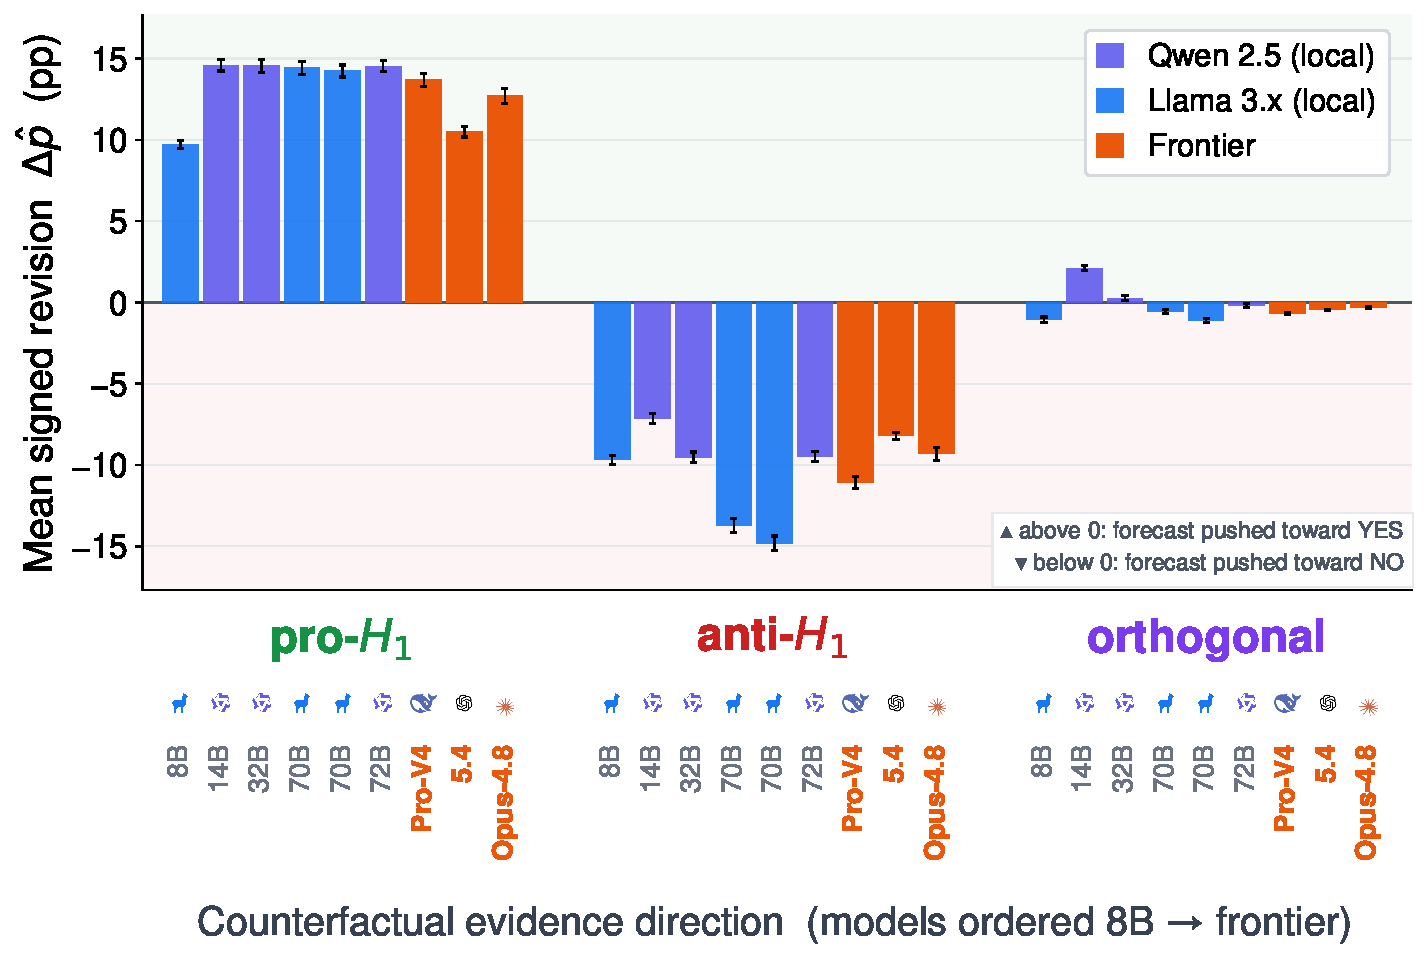
\includegraphics[width=\linewidth]{figures/exp1_direction_selective_updating.pdf}
\caption{}
\label{fig:exp1-bars}
\end{subfigure}\hfill
\begin{subfigure}[c]{0.48\textwidth}
\centering
\footnotesize
\setlength{\tabcolsep}{4pt}
\begin{tabular*}{\linewidth}{@{}l@{\extracolsep{\fill}}ccc@{}}
\toprule
\textbf{Model} & \textbf{EHC$_{\geq3}$}$\uparrow$ & \textbf{HFC$_{\geq3}$}$\uparrow$ & \textbf{Sens.}$\uparrow$ \\
\midrule
\micon{claude.png}~Opus~4.8 & \cellcolor{cellgood!80!cellbad}.990 & \cellcolor{cellgood!80!cellbad}.990 & \cellcolor{cellgood!80!cellbad}$24.0\times$ \\
\micon{openai.png}-5.4 & \cellcolor{cellgood!77!cellbad}.987 & \cellcolor{cellgood!78!cellbad}.987 & \cellcolor{cellgood!23!cellbad}$8.2\times$ \\
\micon{deepseek.png}~V4-Pro & \cellcolor{cellgood!72!cellbad}.977 & \cellcolor{cellgood!70!cellbad}.977 & \cellcolor{cellgood!25!cellbad}$8.9\times$ \\
\midrule
\micon{llamma.pdf}~3.3-70B & \cellcolor{cellgood!65!cellbad}.965 & \cellcolor{cellgood!61!cellbad}.965 & \cellcolor{cellgood!16!cellbad}$6.4\times$ \\
\micon{llamma.pdf}~3.1-70B & \cellcolor{cellgood!62!cellbad}.961 & \cellcolor{cellgood!57!cellbad}.961 & \cellcolor{cellgood!10!cellbad}$4.6\times$ \\
\micon{qwen.pdf}~2.5-72B & \cellcolor{cellgood!62!cellbad}.963 & \cellcolor{cellgood!59!cellbad}.963 & \cellcolor{cellgood!8!cellbad}$4.2\times$ \\
\micon{qwen.pdf}~2.5-32B & \cellcolor{cellgood!62!cellbad}.964 & \cellcolor{cellgood!60!cellbad}.964 & \cellcolor{cellgood!5!cellbad}$3.2\times$ \\
\micon{qwen.pdf}~2.5-14B & \cellcolor{cellgood!48!cellbad}.943 & \cellcolor{cellgood!44!cellbad}.943 & \cellcolor{cellgood!4!cellbad}$2.9\times$ \\
\micon{qwen.pdf}~2.5-7B & \cellcolor{cellgood!17!cellbad}.906 & \cellcolor{cellgood!15!cellbad}.905 & --- \\
\micon{llamma.pdf}~3.1-8B & \cellcolor{cellbad}.887 & \cellcolor{cellbad}.887 & \cellcolor{cellbad}$1.9\times$ \\
\bottomrule
\end{tabular*}
\caption{}
\label{fig:exp1-table}
\label{tab:consistency}
\end{subfigure}
\caption{\textbf{Direction-selective updating across ten models and 38,730 valid update
records.} \textbf{(a)} Mean signed forecast revision by counterfactual direction;
error bars are standard errors. \textbf{(b)} Directional consistency and relevance
sensitivity. EHC and HFC are conditional directional-correctness rates among
movements of at least three percentage points; unconditional results and a
0/1/3/5-pp sweep appear in Appendix~\ref{app:exp1-threshold-robustness}.
Sensitivity is mean directional divided by mean orthogonal absolute revision;
the Qwen~2.5-7B ratio is omitted because its archived revisions mix probability
scales.}
\label{fig:exp1-updating}
\end{figure}

\textbf{Directional packets move forecasts in the registered direction.}
Across 38,730 valid updates, conditional EHC and HFC range from .887 to .990
(Figure~\ref{fig:exp1-updating}). The three frontier agents exceed .97 on both
metrics. Their unconditional directional correctness is 97.3--98.4\%; the
3-point conditional metric omits 6.9--18.1\% of relevant updates that move less
than the threshold. Because the prompt requires $\hat p=P(H_1)$, agreement between
EHC and HFC mainly verifies compliance with that output contract rather than a
second reasoning step (Appendix~\ref{app:exp1-threshold-robustness}).

\textbf{Orthogonal packets produce smaller revisions.}
Frontier sensitivity ranges from $8.2\times$ to $24.0\times$: the same agents move
farther under pro- and anti-$H_1$ packets than under orthogonal packets. Every
scale-valid local model shows the same ordering, with sensitivity from
$1.9\times$ to $6.4\times$.
The result is therefore not confined to the frontier systems, although selectivity
is weaker in the smaller open-weight models.

These results reject an update policy that reacts equally to any
news-like text about the market. They remain compatible with reading the packet's
explicit polarity and applying a learned numerical shift. Experiment~2 removes
that direct mapping: its qualitative cue is informative only when connected to
numerical reference cases.
